\chapter{SM}
Dette afsnit beskriver designet af styringsmodulet, SM.
\section{Klassens ansvar}
Styringsmodulet har til ansvar at holde styr på levelsensoren og værdierne fra VBTE. Den kommunikere med KI og VBTE med indbyggede API'er fra Cypress PSoC 5 biblioteker. 
\section{Klassediagram}
Nedenfor ses klassediagrammet for SM. Bemærk at koden dog er i C men for overblikket er der lavet klassediagram.
\begin{figure}[H]
\centering
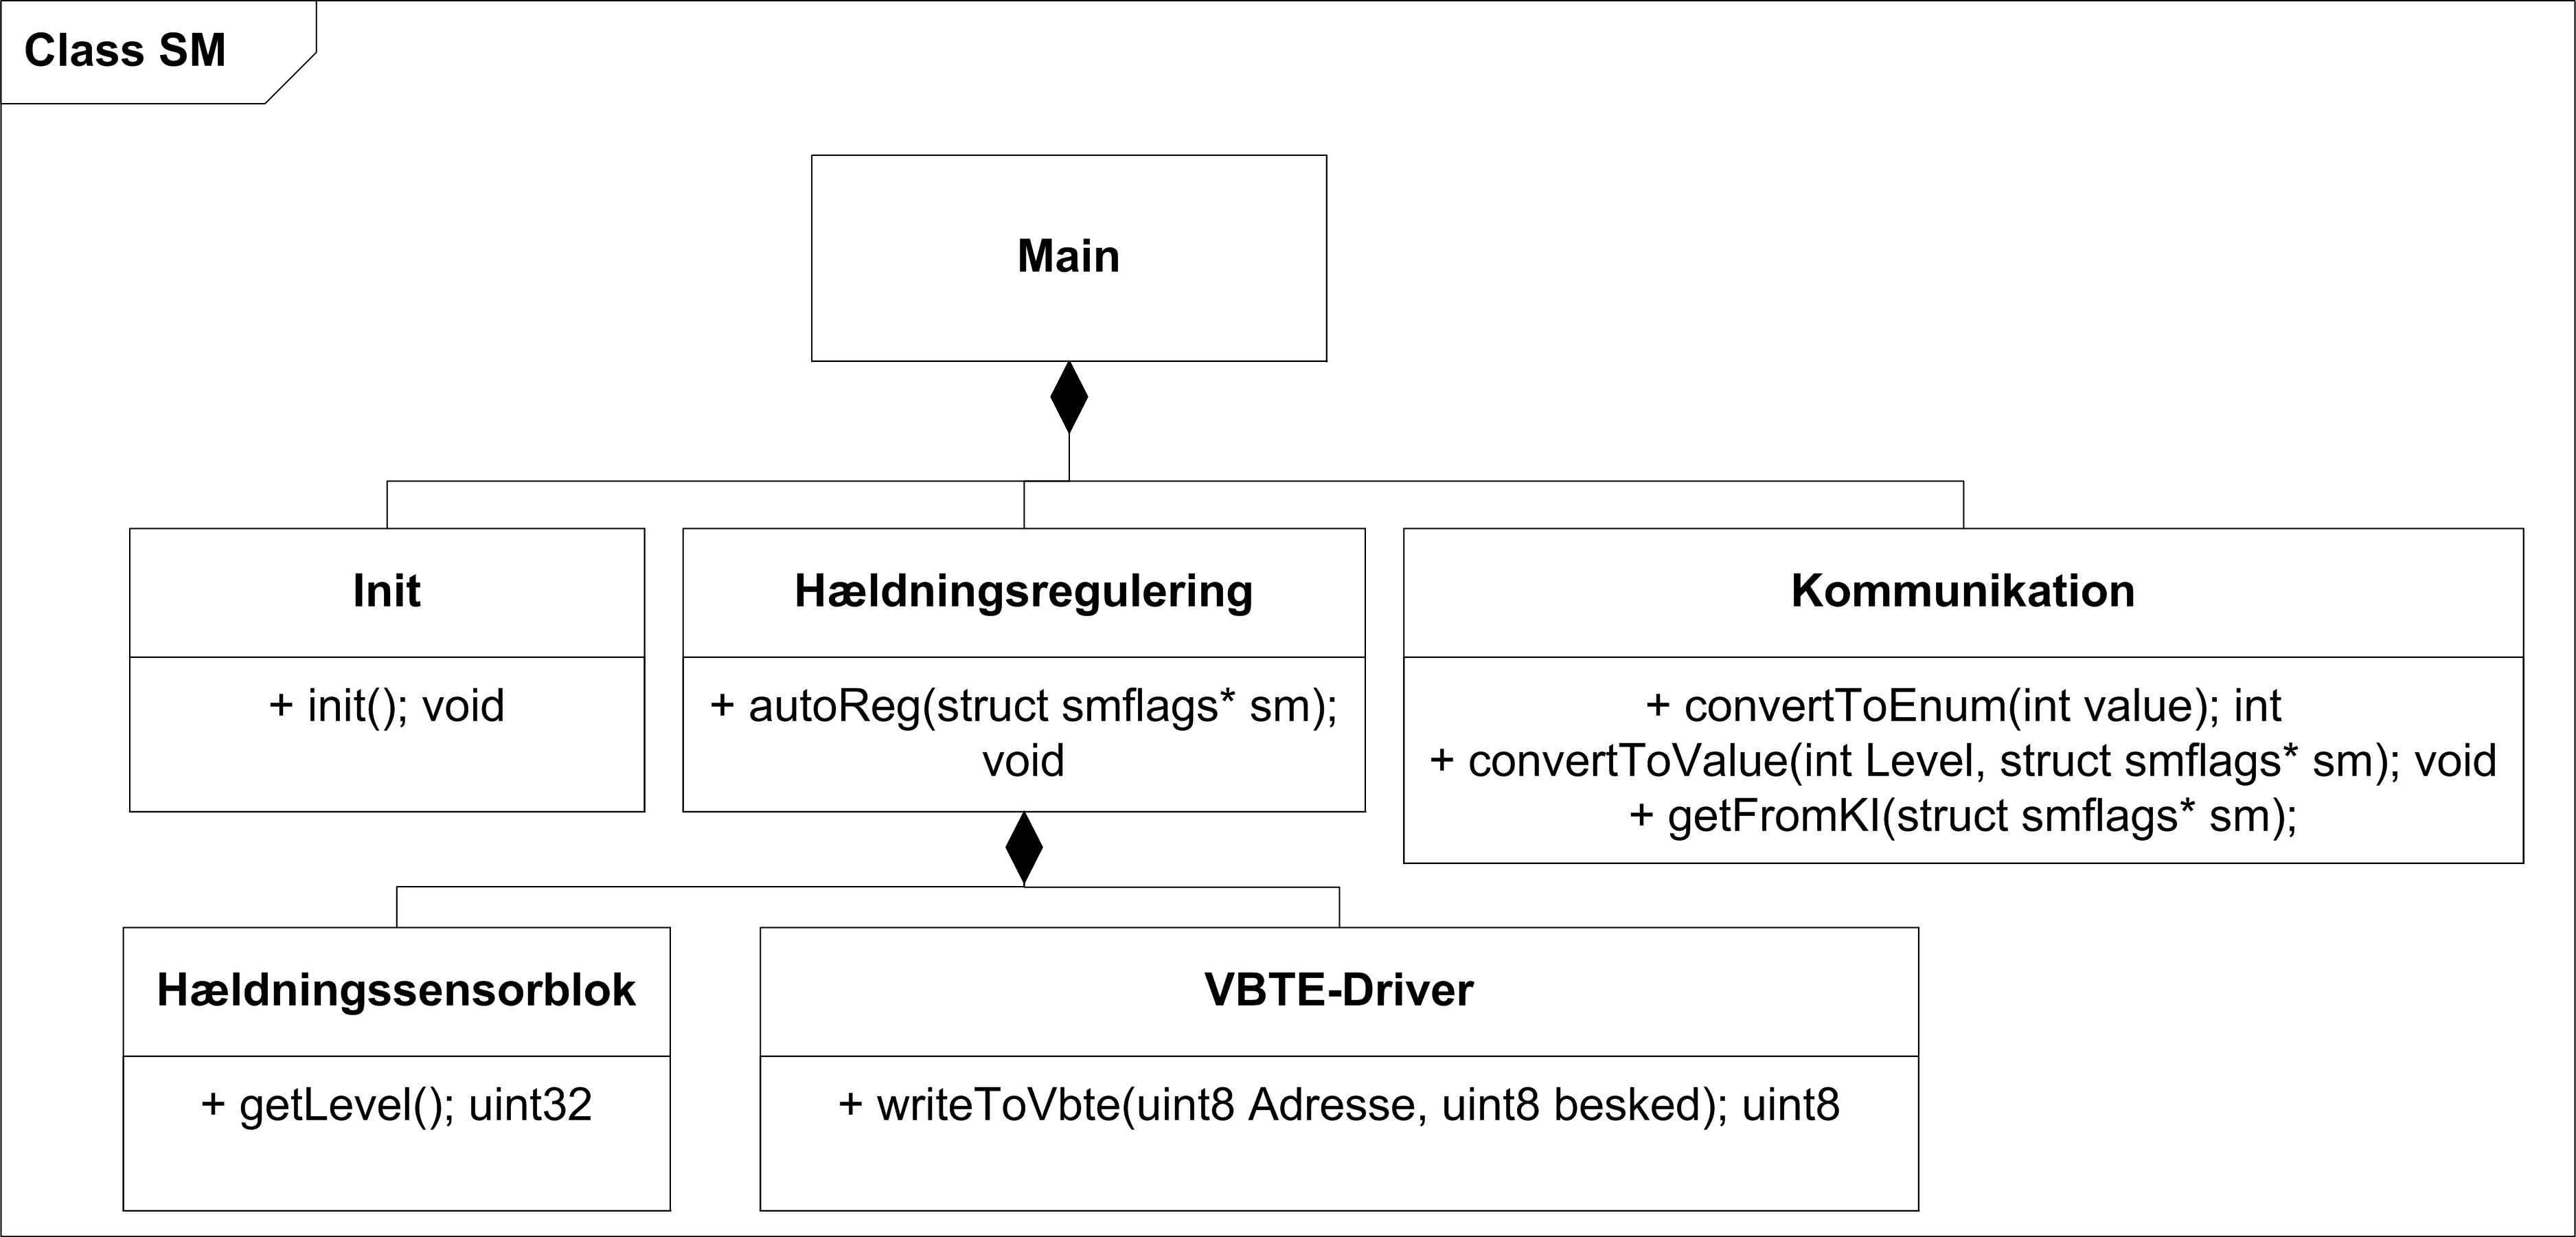
\includegraphics[width=1\textwidth]{billeder/smKlassediagram}
\caption{På figuren ses klassediagrammet for SM}
\end{figure}
\section{Funktioner}
bla bla
\section{Variabler}
\begin{table}[H]
\begin{tabular}{|l|p{10cm}|}
\hline
\cellcolor[gray]{0.8}\textbf{Variabel} &\cellcolor[gray]{0.8} \textbf{Beskrivelse}\\ \hline
autoflag & Denne variable er et flag der holder styr på automatisk regulering .\\ \hline
manuflag & Et flag til at holde styr på manuel regulering.\\ \hline
levelVal & En variable med vores level værdi.\\ \hline
VBTE1Niveau og VBTE2Niveau & Holder styr på vandniveauet i ballasttanke i \%. \\ \hline
VBTE1Status og VBTE2Status & Holder styr op tilgængelighed for VBTE1 og 2.\\ \hline
vinkelVal & Indeholder værdien for manuel regulering.\\ \hline
\end{tabular}
\end{table}
Alle variabler er indkapslet i en struct navngivet "smflags".
\section{Funktionsbeskrivelser}
\subsection{Init}
\subsubsection{Ansvar}
Denne header har til ansvar at sørge for alle komponenter opretter og initieret.
\textcolor{blue}{void} init( \textcolor{blue}{void}); 
\begin{table}[H]
\begin{tabular}{l p{12.5cm}}
\hline
Beskrivelse:& Funktionen anvender API'et fra Cypress componenter og står for at initiere og starte vores PSoC hardware. Den sætter også et register tilhørende vores Accelerometer. \\
Parametre:&ingen\\
Returværdi:&ingen\\
\end{tabular}
\end{table}
% spacer %
\subsection{Levelsensor}
\subsubsection{Ansvar}
Denne header har til ansvar at hente levelværdien ind fra vores accelerometer.
\textcolor{blue}{uint32} getLevel( \textcolor{blue}{void}); 
\begin{table}[H]
\begin{tabular}{l p{12.5cm}}
\hline
Beskrivelse:& Funktionen anvender API'et fra Cypress componenter og venter på at vores ADC henter convertere det analoge signal. Funktionskald for ADC ses i PSoC databladet. \\
Parametre:&ingen\\
Returværdi:&\textcolor{blue}{uint32} levelVal\\
\end{tabular}
\end{table}

\subsection{autoReg}
\subsubsection{Ansvar}
Denne header har til ansvar at 
\textcolor{blue}{void} autoReg( \textcolor{blue}{struct} smflags* sm); 
\begin{table}[H]
\begin{tabular}{l p{12.5cm}}
\hline
Beskrivelse:& ingen\\
Parametre:&\textcolor{blue}{struct} smflags* sm\\
Returværdi:&ingen\\
\end{tabular}
\end{table}

\subsection{I2C\_Kom}
\subsubsection{Ansvar}
Denne header har til ansvar at 
\textcolor{blue}{uint8} writeToVbte( \textcolor{blue}{uint8} Adresse, \textcolor{blue}{uint8} besked); 
\begin{table}[H]
\begin{tabular}{l p{12.5cm}}
\hline
Beskrivelse:& ingen\\
Parametre:&\textcolor{blue}{uint8} Adresse\\
 &\textcolor{blue}{uint8} besked\\
Returværdi:&\textcolor{blue}{uint8} VbteNiveau\\
\end{tabular}
\end{table}

\subsection{KI\_KOM}
\subsubsection{Ansvar}
Denne header har til ansvar at .\\
\textcolor{blue}{void} convertToEnum( \textcolor{blue}{int} value); 
\begin{table}[H]
\begin{tabular}{l p{12.5cm}}
\hline
Beskrivelse:& ingen\\
Parametre:&\textcolor{blue}{int} value\\
Returværdi:&ingen\\
\end{tabular}
\end{table}
\textcolor{blue}{void} convertToValue(\textcolor{blue}{int} Level,   \textcolor{blue}{struct} smflags* sm); 
\begin{table}[H]
\begin{tabular}{l p{12.5cm}}
\hline
Beskrivelse:& ingen\\
Parametre:&\textcolor{blue}{int} Level,\\
 &\textcolor{blue}{struct} smflags* sm\\
Returværdi:&ingen\\
\end{tabular}
\end{table}
\textcolor{blue}{void} getFromKI( \textcolor{blue}{struct} smflags* sm); 
\begin{table}[H]
\begin{tabular}{l p{12.5cm}}
\hline
Beskrivelse:& ingen\\
Parametre:&\textcolor{blue}{struct} smflags* sm\\
Returværdi:&ingen\\
\end{tabular}
\end{table}

\section{Eventuelle Sekvensdiagrammer og state machines}
Måske kommer de senere?